\chapter{Data Collection} \label{chap:data}

As described in Section \ref{sec:ageDB} there are many age-based databases of facial images. However, all existing datasets are based on real age estimation. 

The idea of this work is to compare the performance between predicting real or apparent age labels. In order to do so, a web-based application has been developed using \textit{Facebook's API} to collect a database with these annotations.


\section{Web Application}

The aim of the web-based application was to speed up the collection and labelling processes and reach more people with broader backgrounds to create an age database as diverse as possible. These processes were implemented in a gamified \footnote{Gamification is the use of game thinking and game mechanics in non-game contexts to engage users in solving problems and increase users' self contributions. \cite{Deterding:2011:GDE:2181037.2181040}} fashion so the experience of the users with the application was satisfactory and engaging. 

The application uses the API of Facebook to create a ranking with the user's Facebook friends and add a factor of competitiveness to the game, and also to collect information about the labellers such as gender, age and nationality.

\begin{figure}[!h]
	\centering
	\begin{subfigure}[b]{0.3\textwidth}
		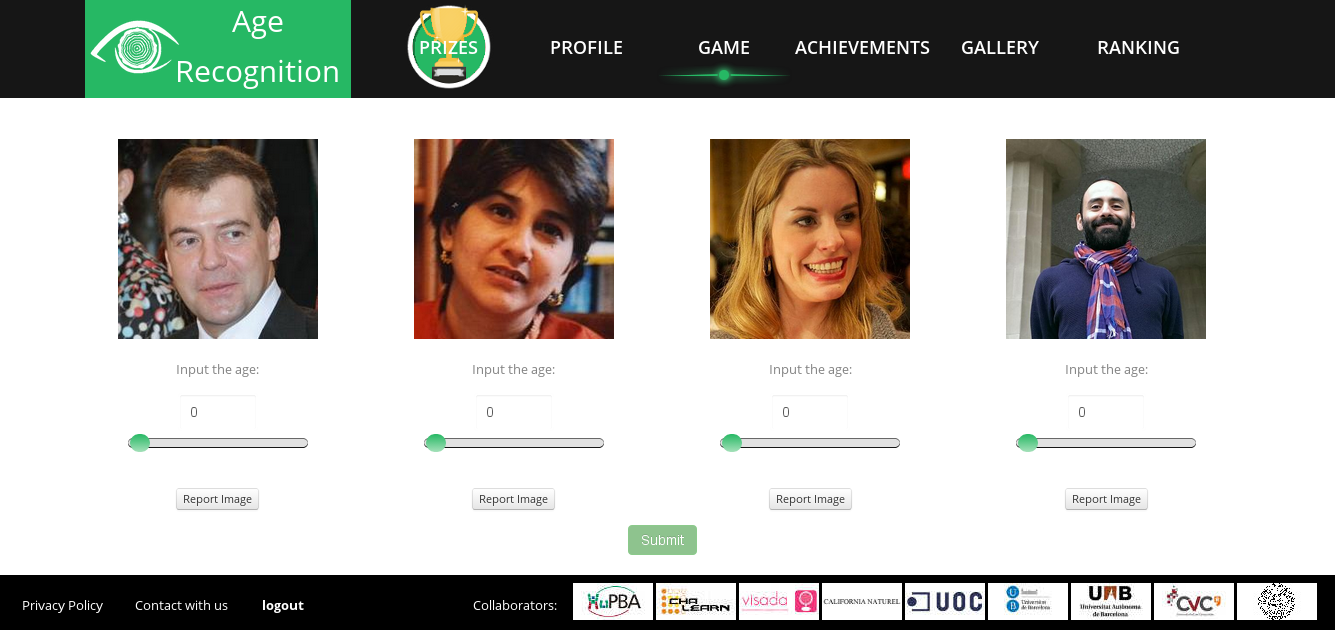
\includegraphics[width=\textwidth]{figures/age_app_1}
		\caption{Game Panel}
		\label{fig:game}
	\end{subfigure}%
	~ %add desired spacing between images, e. g. ~, \quad, \qquad, \hfill etc.
	%(or a blank line to force the subfigure onto a new line)
	\begin{subfigure}[b]{0.3\textwidth}
		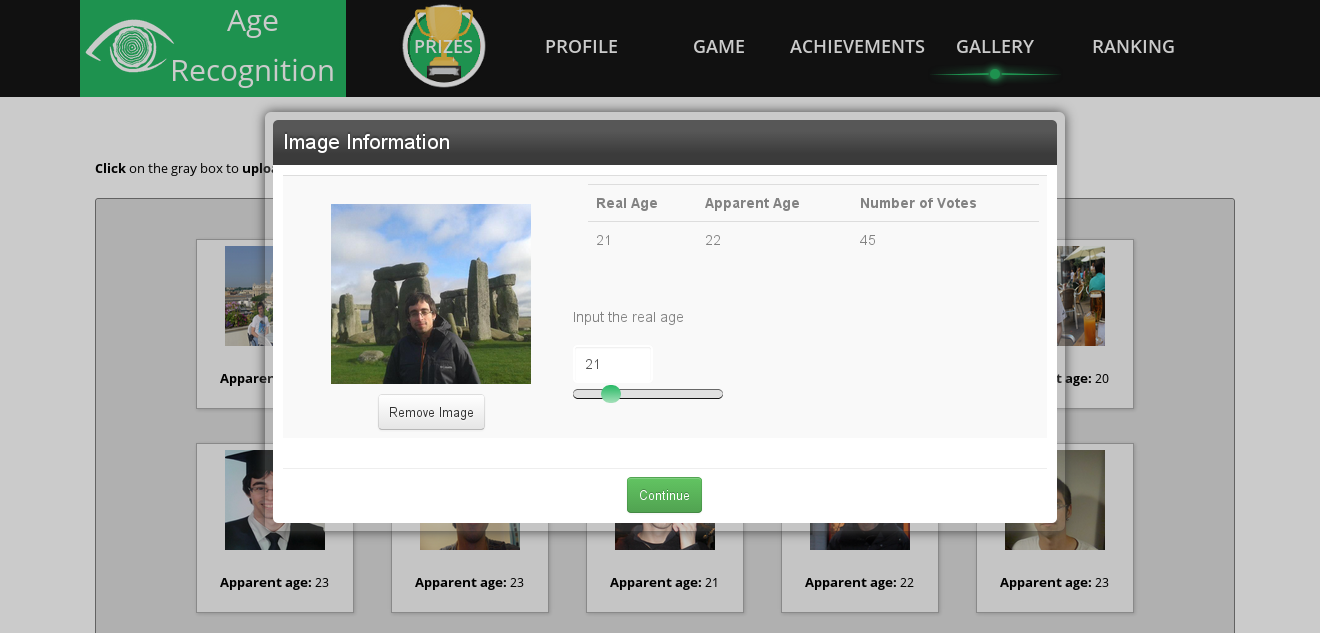
\includegraphics[width=\textwidth]{figures/age_app_2}
		\caption{Gallery Panel}
		\label{fig:gallery}
	\end{subfigure}
	~ %add desired spacing between images, e. g. ~, \quad, \qquad, \hfill etc.
	%(or a blank line to force the subfigure onto a new line)
	\begin{subfigure}[b]{0.3\textwidth}
		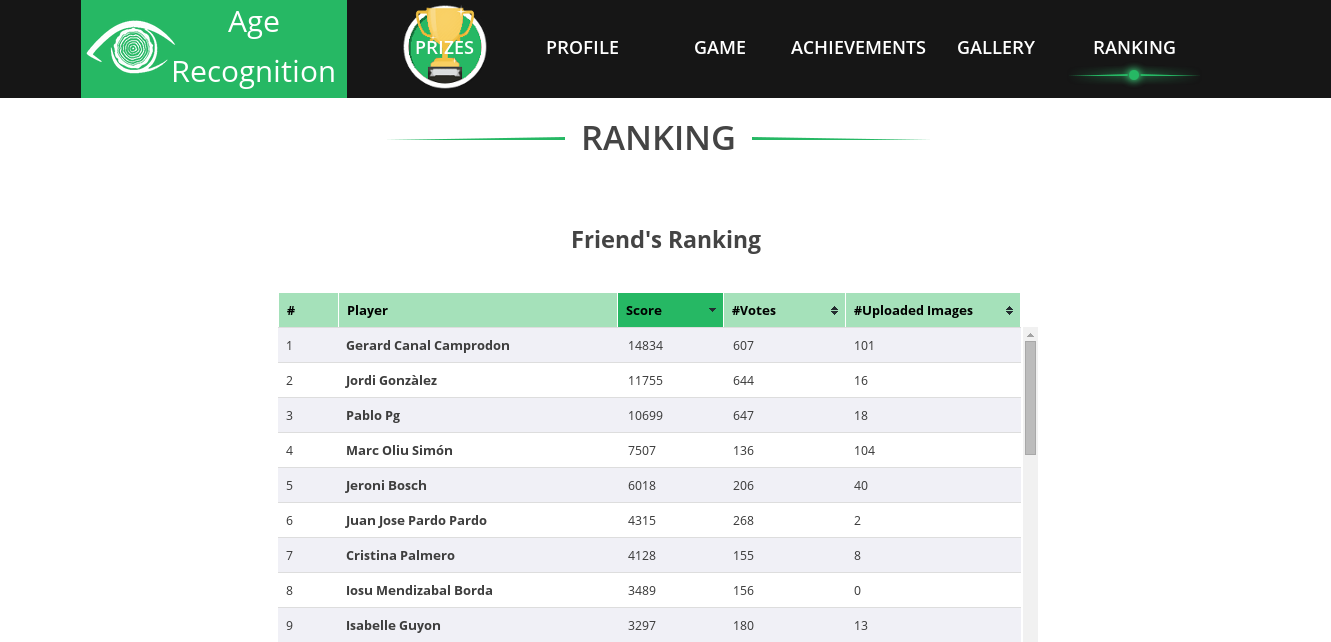
\includegraphics[width=\textwidth]{figures/age_app_3}
		\caption{Ranking Panel}
		\label{fig:ranking}
	\end{subfigure}
	\caption{Age Recognition Application.} \label{fig:application}
\end{figure}

\subsection{Gamification Strategy}
The web-application is basically a platform to label and upload images, which is not funny or motivating. However, using gamification techniques the labeller engagement can be increased. The gamification strategies used were mainly three:

\begin{itemize}
	\item The users or players get \textbf{points} for uploading and voting (labelling) images. The closer the vote is to the apparent age (average current voted age) the more points the player gets. This strategy is pretended to persuade the users to wrongly label the images.
	\item Two \textbf{ranking} tables are shown to the users, one with the ranking positions of the users' Facebook friends and another showing the global classification. This strategy was created with the purpose of increase engagement between users, making them compete with each other. 
	\item A system of \textbf{achievements} was implemented, including the four types of achievements shown in the Table \ref{tab:achiev}.
	\begin{table}[!h]
		\centering
		\begin{tabular}{l|l}
			\textbf{Achievement} & \textbf{Description} \\ \hline
			Share it! &	Invite your friends to play and you will get stars.	\\
			Precision &	The better your guesses, the higher your rank. \\
			Vote! &	Vote on more images to get more stars.\\	
			Add Pictures! &	Upload more images to get more stars. \\
		\end{tabular}
		\caption{List of achievements with its description}
		\label{tab:achiev}
	\end{table}
	\item Thanks to one of the Challenge sponsors, California Naturel \footnote{\url{http://www.californianaturel.com/}}, a bunch of cosmetic lots were offer as a \textbf{prize} for the ones who lid the global ranking. The aim of the prize was to push participation further.
\end{itemize}


\subsection{Application Structure}
When the users access the web for first time they have to register using their Facebook account and accept the terms and conditions for the application usage (further explanation of the legal terms in the Subsection \ref{sec:trouble}). After registration the \textit{How to play} panel will be displayed giving a short description of all the parts of the application.

As it is shown in the Figure \ref{fig:application}, at the top of the site, there is a control menu that allows the users to move through all the site with just one click. A description of the different panels is written below:

\begin{itemize}
	\item \textbf{Profile}: In this section the users can keep track of their statistics (Number of uploaded images, number of votes, points obtained and global ranking position).
	\item \textbf{Game}: This is the main section (Figure \ref{fig:game}), four images are shown at the same time and the users are asked to guess the age of all of them. They can report the images if any of them is considered offensive, bad quality, more than one person appear in the image, etc.
	\item \textbf{Achievements}: In this panel the users can keep track of their achievements and shows the next goals.
	\item \textbf{Gallery}: In this section (Figure \ref{fig:gallery}) the players are able to see the images they have uploaded and see how many people have voted on them and get an estimation of the people opinion. They are also able to upload new images in this panel, while uploading they are asked to crop (if necessary) and specify the real age of the person in the image.
	\item \textbf{Ranking}:	The last panel (Figure \ref{fig:ranking}) allows users to compare their scores with their Facebook friends in the \textit{Friends Ranking} and to all the players in the \textit{Global Ranking}.
\end{itemize}

\subsection{Troubleshooting}\label{sec:trouble}
\note{Add}

We ask the users to upload images of a single person and we give them tools to crop the image if necessary, we also ask them to give the real age (or as close as possible) of the person in uploaded image, allowing more analysis and comparisons with real age and apparent age.


\section{HuPBA Age Dataset}

\note{Show statistic analysis of the database}

Few weeks after release the application we have already collected near 1000 images and near 10000 votes. These numbers will continue growing in order to generate the future competition. Some of the properties of the database which is being collected with the web application are listed below:

\begin{itemize}
	\item Thousands of faces labeled by many users.
	\item Images with background.
	\item Non-controlled environments.
	\item Non-labeled faces neither landmarks, making the estima-
	tion problem even harder.
	\item One of the first datasets in the literature including
	estimated age labeled by many users to define the ground truth
	with the objective of estimating the age.
	\item The evaluation metric will be pondered by the mean and
	the variance of the labeling by the participants.
	\item The dataset also provides for each image the real age
	although not used for recognition (just for analysis purposes).
\end{itemize}

In the same way for all the labelers we have their nationality, age, and gender, which will allow analyzing demographic and other interesting studies among the correlation of labelers. In relation to the properties of existing datasets shown in Table I, ours include labels of the real age of the individuals and the apparent age given by the collected votes, both age distributions are shown in the Figure 2. The images of our database has been taken under very different conditions, which makes it more challenging for recognition purposes.
